\documentclass{sig-alternate}

\usepackage{hyperref}
\usepackage{cite}
\usepackage{url}
\usepackage{graphicx}
\usepackage{subfigure}
\usepackage{color}
\usepackage{comment}
\usepackage{multirow}
\usepackage{booktabs}

\newcommand{\cm}{\textcolor{magenta}}
\newcommand{\cb}{\textcolor{blue}}
\newcommand{\cred}{\textcolor{red}}
\newcommand{\cg}{\textcolor{green}}

\begin{document}

\hypersetup
{
    pdfauthor={Yan Zhai},
    pdfsubject={CS736},
    pdftitle={Measruing the Linux Virtual Memory Subsystem},
    pdfkeywords={Measuring, Virtual Memory, TLB, Page}
}

\title{Measruing the Linux Virtual Memory Subsystem}

\author{
    \alignauthor Yan Zhai\\
        \affaddr{Department of Computer Science and Technology,
            University of Wisconsin Madison}\\
        \email{\{zhaiyan920\}@gmail.com}
}

\maketitle

\begin{abstract}

   Virtual memory is one of the most important subsystems inside modern operating
   systems. Although it is transparent to users, understanding the virtual memory
   can help to build better applications, especially in performance improvement.
   In this paper, I come to four issues of virtual memory: TLB, User space
   allocator, huge pages, and optimization of code sharing. I use performance
   measurement to explore deeply how these parts are working underlying. Most of the experiments run as I expect, except the TLB part. I will
   explain further in the paper about the methods, the results, and the conclustions
   on each separate parts. Moreover, I will try to illustrate why TLB measurement
   does not work well in some case.

%  In this paper, we find that for BTIO, through tuning the I/O configuration
%  the application performance can be improved 30\% than the default NFS
%  configuration without increasing any extra cost. As the number of I/O servers
%  of the parallel file system increases, the application performance can be
%  improved continuously. 

\end{abstract}

\section{Introduction}
    \label{sec:intro}
    %PVFS\cite{bib:pvfs}, and Lustre~\cite{lustre}.  For a selected parallel
    %\begin{itemize} 
    %    \item 
    %    \item 
    %    \item 
    %\end{itemize}
	
The virtual memory subsystem has become an indispensable constitution in modern
operating systems. With the proper hardware support in paging and segmentation,
operating systems build their own mechanisms of protection and abstractions to
users. This greatly simplifies the price to write correct code, and also make
the operating system more reliable to the user faults.

However, writing correct code is not equal to writing good code. The
applications may not perform well without knowing underlying operating systems
and hardware. For example, designing a good web server will often require good
knowledge of how to maximize the usage of memory and avoid long latency from
disks~\cite{c10k}. Thus, it would be quite attractive to reveal what is beneath
the beautiful illusory operating systems provide with you.

The virtual memory subsystem is quite huge, we mainly focus on several topics:
\begin{itemize}
\item TLB(Translation Lookaside Buffer), the 'cache' of the virtual memory. It
will be necessary to know how the TLB are working, how large it is. We try to
measure the TLB size through a set of experimentations, in order to know more
deep about this small buffer.
\item Huge Pages. To avoid TLB missing, huge pages can serve quite good for
this purpose. But while it has many benefits to use huge pages, what is the
cost? In this paper, I try to illustrate the cost of huge pages with the 
performance cost in page preparation, allocation aspects.
\item Memory Allocator, like \emph{malloc}, \emph{mmap}. The only thing users
can see is these allocators will allocate the virtual pages when invoked. However,
when will the page be actually allocated? What is the allocation policy of the
physical pages? These are all interesting questions to answer.
\item Optimization of Virtual Memory System. There are many optimization for the 
virtual memory, like better page replacement algorithm, prefetching, and so on. In
this paper, I explored the benefits from the object sharing.
\end{itemize}

To flexibly employ all kinds of measurement strategies, I choose Linux as my
major experiment environment. Four major experiments, and several minor ones
are carried out toward above topics, and most of them run well, matching my
understanding to the architecture and system. One thing that causes trouble is
the TLB. The measurement of L2 TLB is not quite accurate, and I will explain the
reasons with the gathered timing and hardware events data.

The paper is organized in following way: section~\ref{sec:timing} will
introduce the environment, including time function I used, and some
configuration details. section~\ref{sec:tlb} is measuring different level TLB sizes.
section~\ref{sec:alloc} describes how I measure the memory allocator. section~\ref{sec:hugepage} will test
the huge page overhead, section~\ref{sec:sharedobj} illustrates the benefits from shared objects.


\section{Experimental Environment}
	\label{sec:timing}
\subsection{Timer in Linux}
To best measure the times in experiments, I still decide to use system call
\emph{gettimeofday}. The major idea behind this is to enlarge the experiment
scale, and ammortize the overhead. There are some high resolution things like
\emph{Rdtsc} instruction on Intel's X86/64 platform. But it's hard to use, and
its behavior varies on different platforms as I tested. Though
\emph{gettimeofday} only supports measurement at ms level, we could see later,
it is enough for our experiments.

\subsection{Hardware and Software Environment}
The machine I used for testing is a x86-64 machine. The processor is Sandy
Bridge family, Intel-i5 2500K 3.3GHZ. This processor has two level private
cache, and a last level shared cache. Both L1 data cache and instruction cache
are 32KB in capacity, 8 way set associative, with 64 byte cache line. L2 cache
is 256KB, also 8 way set associative. The last level cache is 6MB. Ram size is
16GB. The operating system I chose Fedora 17, with the linux kernel version
3.3.4. Compiler version is gcc-4.7.0. I also used a performance tool called
\emph{perf}~\cite{perf}, which operates on hardware performance counter related interfaces.


\section{Measuring TLB size}
	\label{sec:tlb}
TLB is one greatest optimization that makes virtual memory to work faster.
Without TLB, each memory reference will have to do no less than two memory
reference, for actual physical pages associated with, and for the real address
CPU wants to visit. In this section, I try to measure the TLB size on my
machine. The result is not exactly what I expected, and I will try to explain that in the discussion section~\ref{subsec:tlb-discus}

\subsection{Methodology}
To measure the size of TLB, I chose to observe the timing difference on referencing
memory. If the TLB hits, then the reference should be faster than TLB misses
cases. The goal could be achieved if we carefully construct the memory visiting
sequence, then we can find out the thrashing behavior in timing when come to the
point TLB begins to miss. Specifically, if not mentioned, TLB later all
mentions to data TLB.

\subsubsection{Complications}
Correctly measuring TLB size is not an easy task due to following complications:

\begin{itemize}
\item Hardware cache can interference heavily during the walking process. To
be accurate, one needs to distinguish the cache miss event and
TLB miss event. Unfortunately, these two events are usually comparable in missing
penalty, and make things complex. Even worse is that caches are usually physical
associated, and the addresses we can provide at userspace are virtual addresses.
For the set associative caches, if their associative sets number are larger than
the number of cache lines per page, then we can not fully control the cache. And
this in fact causes great trouble when I came to measure the L2 TLB size.
\item Hardware can have mechanism that ruins the assumptions about sequential
programming model, like out-of-order instruction retiring, multiple processing
units, and hardware prefetching and so on.
\item Modern CPU can have multiple level of TLB. On my platform, there is two
L1 data TLB for different page sizes, one L1 instruction TLB, and one shared L2
TLB. We need to let level 1 TLB to miss before we can measure level 2 TLB.
\item Difficulties in generating the correct benchmark. The overhead in
language constructs, operating systems interactions, and the compiler's
aggressive optimizations can all become obstacles to obtain the correct results.
\end{itemize}

\subsubsection{Strategy}
To solve the above complications, I carefully construct my sequence to walk on
memory. First thing is to design a pattern to maximize cache hit. One
observation that helps is: level N TLB (N=1,2) usually has less entries than the total
cache line number in level N cache, but its total size is larger than the corresponding
cache. Due to this fact, we can force level N cache to hit, while level N TLB to miss.

This goal can be achieved by visiting exactly one cache line inside each page.
We first allocate sufficient pages, and gradually increase the number of pages
to walk on.  The phase change point in timing would be approximation size of
TLB size. To make cache hit, the stride we use to walk on pages is sum of page
size and cache line size. This ensures we visit a different set of cache lines
in the next page and will maximize the cache utilization. When it goes off the
page boundary, then just rewind to the start of next page and keep on this
procedure. 

This strategy should work for both L1 and L2 TLB. Actually, by maximize the cache
utilization, at the point of L2-TLB miss, we will observe different timing
behaviors. Let's define $C_i$ to be level i cache hit, $T_i$ to be level i
TLB hit, and $C_m$, $T_m$ to be cache and TLB miss correspondingly. Then we
should observe $C_1T_1$, $C_1T_2$, $C_1T_m$, or $C_1T_1$, $C_1T_2$, $C_2T_2$,
$C_2T_m$. There should not have $C_2T_1$, or $C_mT_2$ behavior, so the timing
curve would be monotonically non-decreasing as we enlarge the walking page size.

Since memory references are tiny things to measure, we repeat the memory walk
many times and measure the average.
%At the beginning I enforced each walk to
%make same number of memory reference, but later I found this is wrong so I
%adjusted to use same iterations for each walk. The reason will be discussed
%in~\ref{subsec:tlb-discussion}

\subsection{Implementation}
The implementation is quite tricky. Firstly I manually unrolled innermost loops
of all walking routines, and ensuring they have the least number of
instructions. This can avoid loop overhead to small loops as well as improve
the hit rate of instruction cache. Additionally, all operands are aligned to same
size to avoid size extending. Before walking, the memory should be warmed
several times and evict out dirty data. The last thing then come with the
compiler optimization. In one hand, we can rely on the optimization to reduce
the uncessary memory visit and computation, rather than manually coding
assembly (actually I did this for some very small walk kernels), but on the
other hand we should add some fake "use" to avoid our code being optimzed out.
Also, inline optimization should not be used abusively. Large chunk of inlined
code can hurt the instruction cache, which is unnecessary overhead.

To automate the experiment, I also write code to measure cache size and
associative sets. I reference the paper here~\cite{sigmetrics:cache}. To avoid
the problem of physically not continuous, I resort to huge pages, and then things
become a lot more easier, just capacity probe suffies to find out how many
cache lines and how many associative sets are in each cache. Due to the space limitation, I won't show the detail here. Further information could be found in~\cite{github}.

\begin{figure}[hpb]
\centering
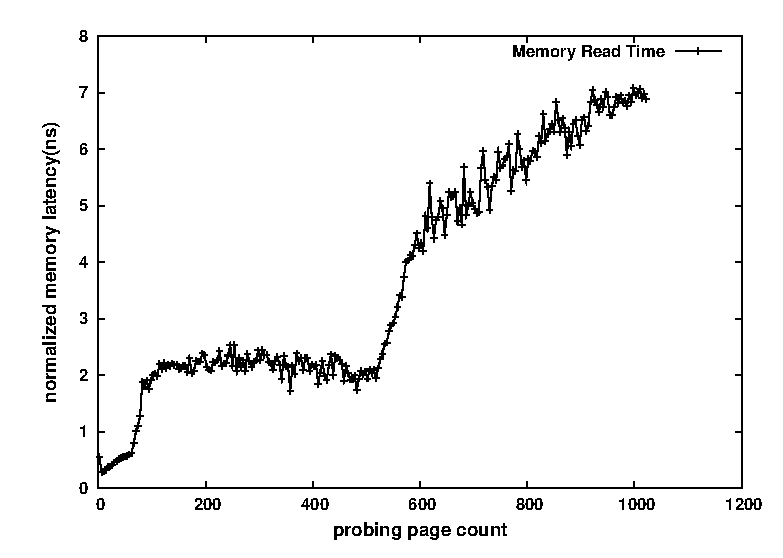
\includegraphics[width=0.9\linewidth]{../figures/time}
\caption{Memory walk time on different number of pages. The stride size I use is 4160 byte, the sum of page size and cache line size, so the memory reference will happen on each page exactly once.}
\label{fig:tlbsz-time}
\end{figure}

\subsection{Experiment Results}

%
%
% 1. cache measuring result
% 2. TLB size measuring result
% 3. huge tlb result
% 4. TLB way measuring
%
%
Figure~\ref{fig:tlbsz-time} shows the timing result of TLB probing. The first
half of the result looks quite reasonable, clear boundary and more stable
than the second half after I have probed about 512 pages.

\begin{figure}[hpb]
\centering
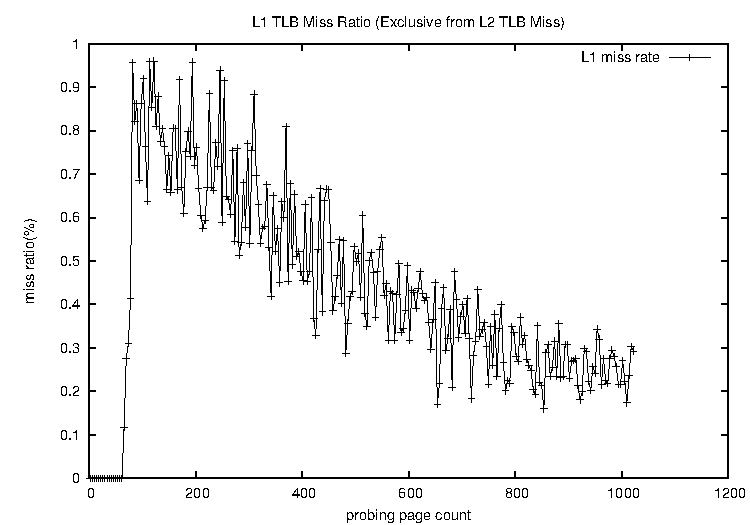
\includegraphics[width=0.9\linewidth]{../figures/tlb}
\caption{L1 TLB miss rate during memory walk, generated by \emph{perf}. The L2 TLB data, however, nearly have no missing all the time no matter how much I used the memory.
}
\label{fig:tlbsz-tlb}
\end{figure}

\begin{figure}[htp]
\centering
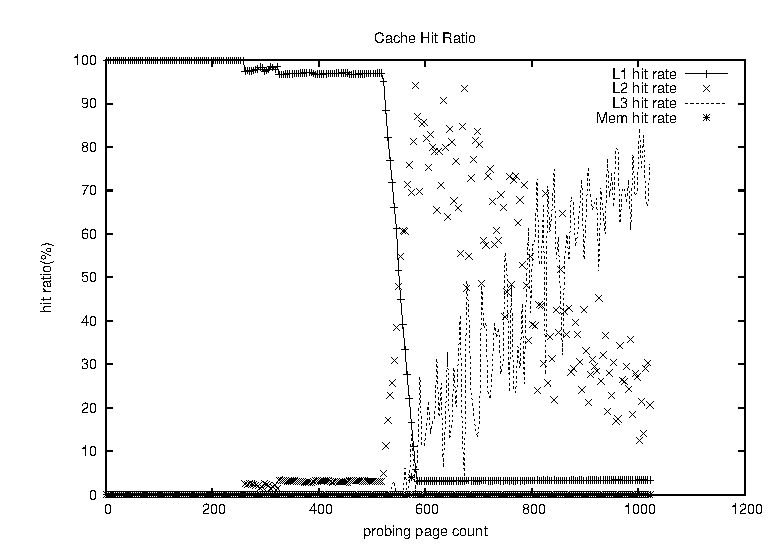
\includegraphics[width=0.9\linewidth]{../figures/cache}
\caption{Multiple level of caches hit ratio. The hit rate for each level is exclusive, i.e. if L2 cache is hit, then L1, L3 miss is not hit. Memory hit simply means memory reference, and this seldom happens}
\label{fig:tlbsz-cache}
\end{figure}

To verify the case, I use \emph{perf} to collect the hardware data. The \emph{perf}
event combined with umask I used are: r1008,dTLB,r01D1,r02D1,r04D1,r20D1. They can
 be found in~\cite{intel-dev3}, section about Sandy Bridge i5-2xxx serial.

From the figure~\ref{fig:tlbsz-cache} and figure~\ref{fig:tlbsz-tlb}, I can
confirm before the page number grows to 512, things are correct, and the
L1 TLB size would be around 64 entries. However, after I reached about 512
pages, it becomes quite unstable. The reason can be found mainly in
figure~\ref{fig:tlbsz-cache}, the L2 cache begins to miss heavily.  The reason
is pages could be non-continuous in physical. I will discuss a possible 
workaround to this problem in section~\ref{subsec:tlb-discus}.

Another annoying fact is that \emph{perf} didn't show me the reasonable L2 TLB
miss number. But from the change of L1 TLB miss rate, which indicates L1 TLB
miss and L2 TLB hit, it's almost reasonable to assume the L2 TLB is also
missing. The reason is quite simple: with my walking sequence, if L2 TLB is not
missing, then L1 TLB either keeps missing on every access, or don't miss at
all. So I don't even need a hardware counter to confirm the correctness, as
long as the L1 TLB data is not also faulty.

\subsection{Discussion}
\label{subsec:tlb-discus}
The first time I used register-base-scale addressing to implement the walk
kernel. However, this is not quite good choice. The reason is even CPU miss
on a TLB visit, it can still issue following instructions because there are
no data dependency, and the overhead is amortized so that phase change is
not clear, even if I have observed high TLB miss rate and cache hit rate.

The next method I tried was linked list. Within each cache line I encode the
next address to visit and make it a linked list. In this way, the phase change
becomes more outstanding when I increase the probing page count by factor 2.
However, if I increase probing count by adding 1, then the normalized time for
one memory reference exhibits the above behavior. The reason to blame for is
the potential of non-continuous physical page. On my platform, there will be
512 cache sets on L2 cache, which means, if using 4KB page, 3 higher bit used
to reference the cache sets will not be controllable by users. Operating system
can even enforce the cache separation by not allocating physical pages with
certain set index to users. The problem here is, although in theory we could
probe more than 4096 (8-way 512 sets) pages before L2 cache misses, in practice
only 512 (8-way and 6-bit sets) can ensure visiting without miss.

But on the other hand, assume operating systems are not restricting users'
control on cache lines, then an interesting observation may help workaround this
problem. That is, the chances for 8 pages having same high 3-bit index are rare.
So we can change the walking algorithm to:
\lstinputlisting{tlb.c}

Testing whether can add a new page is to test whether walking on same cache
line in that set can cause L2 cache miss. When we found enough pages, we can
link these pages together and walk to check timing. I haven't got time to
derive the actual expectation, but it should be much larger than the current
turning point 512. I have implemented a prototype for this algorithm, but not yet tested due to time limit. 

In my experiments, I didn't measure the size of huge page TLB. One reason is it
is gradually become unified TLB, and measures the small page TLB should be
enough in future.  On the other hand, the whole thing required to measure huge
TLB would be similar as above process, and much easier since L2 cache sets are
all embodied inside the continuous huge pages.


\section{Memory Allocator}
	\label{sec:alloc}
Memory allocator is a major interface that operating systems exposed to the
users. On Linux, users request memory throught the system call \emph{brk} or
use the memory mapped file through \emph{mmap}. This can also be unified by
standard library interface \emph{malloc}.  The operating system, will ensure
that if the requests are granted, then visiting these address would not cause
protection errors and thus can be used by user applications. However, this does
not mean operating system will allocate the physical page, say, setting up the
virtual page to physical mapping immediately.  Rather than fit user's request
once and for all, operating systems may employ a lazy allocation strategy. In
this configuration, only when a page fault occurs, will the operating system
check the need to allocate physical memory. In this section, I verify three things.
First is that whether operating system uses on-demand allocation, and second
is when will operating system zero out the pages for security concerns. At last
I will verify the benefit of on-demand allocation.

\subsection{Methodology}
The strategy I used is quite simple. To determine whether operating systems
allocate pages on demand, we just allocate a large memory area, and visit the
performance we walk upon first time. It should be quite different than normal
walking. To further distinguish what operating systems are doing, I will measure
the time with and without allocating system call, here I used \emph{mmap}, as
well as the normal walk time.

To check when does operating system zero out the pages, if the allocation is
not done at the system call time, then it's only possible for operating system
either to 1.) choose a known zero page 2.) zero out page on demand. In order
to exclude or include the first approach, I measured the time of allocation
both when free memory is abundant and is scarse. I try to make sure that 
operating system will not have many free zero pages to borrow, then I could
figure out whether there will be extra cost during allocation. One problem may
still remain is that kernel can zero out pages when pages are unmapped. So I
also measure the normalized time used to unmap a clean page and a dirty page.

\subsection{Experiments}
\subsubsection{Allocation Cost}
\begin{figure}[htpb]
\centering
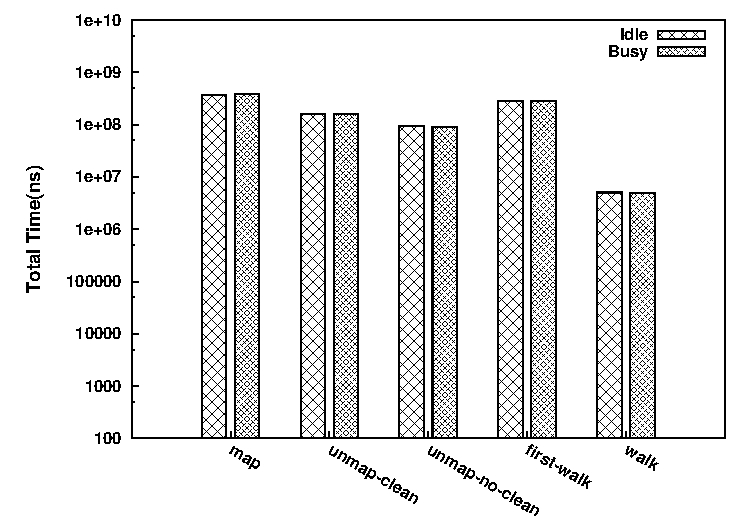
\includegraphics[width=0.9\linewidth]{../figures/alloc}
\label{fig:alloc}
\caption{The different part of allocation time. \emph{map} means the entire time
including the mapping, walking, and unmapping. \emph{unmap} has two options, to
zero out the page (suffixed with "-clean"), and don't do extra things (suffixed
with "-no-clean"). The first walk means the duration of the first time we visit
the allocated space, and walk means the time to do memory walk after we have
touched all the pages several times.}
\end{figure}
To address questions we mentioned, I measured several parts of the overhead in 
figure~\ref{fig:alloc}:
\begin{itemize}
\item total overhead (tagged as "map-full"). Including mapping, memory walking
and unmapping time.
\item first time walk overhead. This will ensure the pages be allocated.
\item unmapping overhead, with/without reset routine. Measuring this part is
for the sake to explore if operating systems can do zero out at reclaim time.
\item regular memory walk after all the pages are assured to exist in memory(I
monitored the swap space used, and it's not grown at any experiment time).
\end{itemize}
These experiments are done under memory idle period, and memory pressure
period. To compare the zero-out strategy, we also measured the allocation
time when memory is scarse resource. In this scenario, the free memory I leave
to operating system is less than 1.5GB, and the allocation unit I used is
1GB, to make sure few free pages are in the system, and it must zero out pages
at the time of granting or revoking them to users.

From figure~\ref{fig:alloc} we can easily find out the allocation is on demand, since regular
walking is much too cheap comparing with the first time memory walk after
mapping a set of memory. And also the performance retains regardless of the
memory pressure. According to that fact, it is only reasonable to zero out
pages on allocation and deallocation time. But the measurement of unmapping
time did not show much information, since the unmapping time is sufficiently
large that we can not distinguish that if it actually does page zero out.

\subsubsection{Benefit from On-Demand Allocation}

\begin{figure}[htb]
\centering
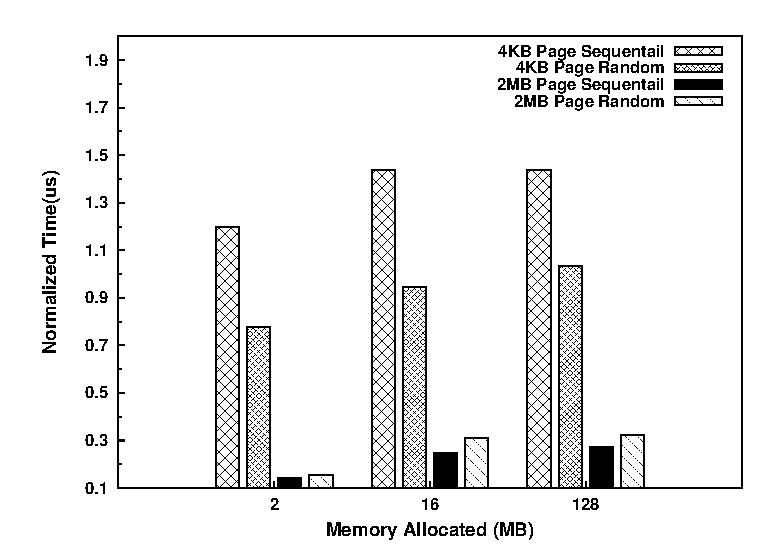
\includegraphics[width=0.8\linewidth]{../figures/on_demand_4k}
\label{fig:on-demand}
\caption{The different of doing random walk and sequential walk through the 
newly allocated 128MB memory. For small page space, random walk would not bring
in the page not needed, thus performs better than sequential walk. But for
large page space, random walk is slower.}
\end{figure}

The on demand allocation is an optmization for virtual memory. To see its
effect, I compared the cost to do random walking and sequential memory walk
on the 128MB newly allocated memory. For space limitation, I only present the
result on 4Byte stride as in figure~\ref{fig:on-demand}. Further results are
uploaded to~\cite{github}, it is consistent with my conclusions here.

Figure~\ref{fig:on-demand} exhibits interesting result: random walk runs
faster with small pages, but slower with large page. In the former case,
don't not bring in unnecessary pages save time, while in later one there
is no much pages to bring in, and poor locality slows it down.

\subsection{Discussion}
One thing hard to illustrate is whether operating system will 'smartly'
allocate some pages for small requests. For example, when user requests for
only 1 page, then allocate the page immediately to avoid a page fault can be
somewhat a good choice. This period is too small to measure correctly just by
using wall clock. However, if the operating system can provide a page fault
counter for each process, then it is still possible to measure such behavior.
Due to both the time limit and space limit, I didn't implement this as part of
the benchmark.

\section{Huge Pages}
	\label{sec:hugepage}
Huge pages are an optimization for performance. On latest Intel x86-64
platform, the page size can be even 1GB. This provides good chance for
applications to tune their performance, like the databases, or the host mode
virtual machine monitors. The benefits of huge pages have been long mentioned,
but viewing from the virtual memory system, it can be cost, like to prepare
these huge pages will rearrange memory so it is physical continuous. Moreover,
when page fault happens, it's much heavier than small page faults. In this
section, I try to show the cost of huge pages.

\subsection{Methodology}
The experiments focuses on the cost of allocating huge pages. Preparation time
can be quite long, but it is a one time cost, and will be much less possible to
become a bottleneck. So I will care more about what happened during using the
huge pages. What I did was allocating same amount of memory using both large
and small pages, and comparing the time elapsed with both sequential walking,
and random accessing. Also, I will increase the walking iteration, so that I
can find out what frequency of use can make huge pages competitive in
performance , even it has much larger overhead to be set up and zeroed out.

\subsection{Experiments}

\begin{figure}[hbt]
\centering
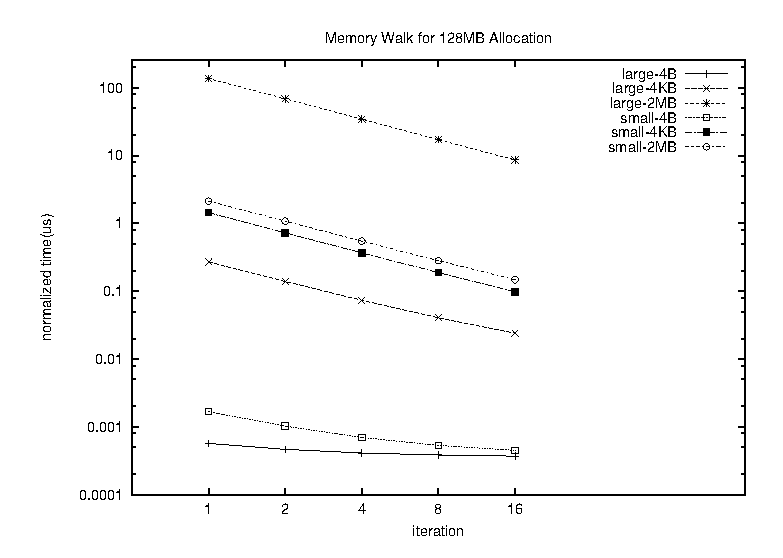
\includegraphics[width=0.9\linewidth]{../figures/hugetlb_128m}
\caption{Memory walk time on 128MB mapped memory. I use different stride, and
iterations for each walk, and measure the average time cost. The larger the 
stride size is, the worse performance I will get by using huge pages. Due to
space limitation, I didn't draw more stride result. Actually the small page
start to beat huge ones from the point of 32KB stride.}
\label{fig:hugetlb-time}
\end{figure}
\begin{figure}[h]
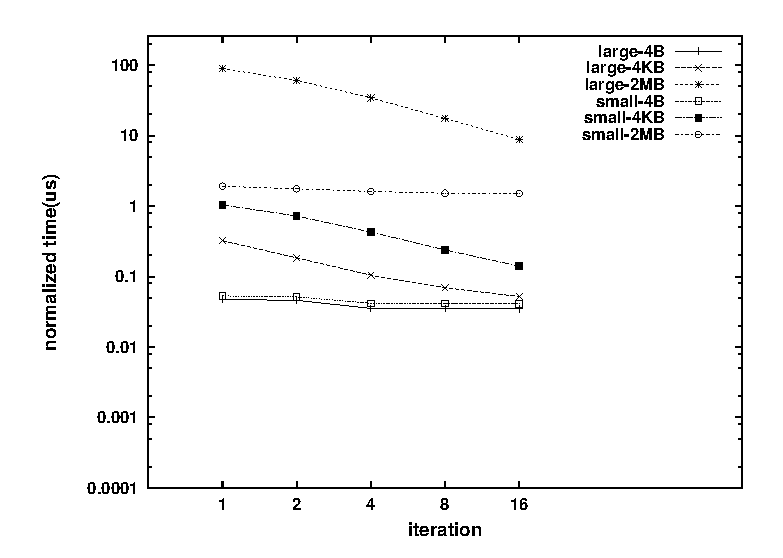
\includegraphics[width=0.9\linewidth]{../figures/hugetlb_rand_128m}
\caption{Random walking is similar with sequential walking, when in small stride
size the huge pages perform better. Here the stride is just used to determine
the amount of memory reference, rather than walk pattern. I use stride to label
it for comparison with sequential walk. One thing changes in random walk is
that for 4B stride, both of the two configurations perform worse than
sequential walk. The reason may be related with locality, but it is not what we
address here.}
\label{fig:hugetlb-rand}
\end{figure}

Figure~\ref{fig:hugetlb-time} shows the cost of walking on newly allocated
small and huge pages, total memory size is 128MB. The stride we used to walk on
the pages are from 4B to 2MB, with multiple iterations in each walk. It is quite
clear that huge pages performs bad when iteration number is small, and stride
is large. With the iteration increasing, its average performance becomes better.

Random walking shows similar trend as in figure~\ref{fig:hugetlb-rand}. Small
pages still perform better at the beginning, but normalized difference is
smaller. The result again illustrates the benefit of on demand allocation:
setting up the mapping and zeroing out pages at the very beginning is not a must, since the applications may not reference them all.

\subsection{Discussion}
Although there are some inconveniences, huge pages are useful, especially
when used by VMM. If no huge pages are used, then on a 4 level paging system, a
page fault can require up to 20 times memory reference. With the huge pages,
this can be reduced to minimum. The problem for the huge page is that it must
be configured and requested explicitly, thus may lead to memory pressure.
Another thing is the recognition of the cost of huge pages: for large data not
frequently referenced, using large pages may not get benefits.

During experimentation, I found a strange thing:in Linux normal users can get
huge page through \emph{mmap} interface using anonymous mapping, without
causing protection errors. However, the similar access through \emph{shmget}
interface will not work, unless super user privilege is granted. I didn't see
any differences between these two approaches, hopefully it is not a security hole.

\section{Shared Code Page}
	\label{sec:sharedobj}
Shared code pages is an important optimization to the virtual memory. Previously
I have shown the benefits from demand allocation as an optimization, now I will
go on exploring the shared library, or shared object.  Shared code usually
appear as shared library or dynamic linking library in the system.  With shared
library, code size are largely reduced.  Moreover, the shared library is
usually place independent and can be dynamically loaded by the applications.
This enables great flexibility in design. For instance, apache~\cite{apache}
uses dynamic libraries to implement its modules, which can be loaded on demand
and built separately. In this section I focus comparing the typical
applications' code size by linked them statically and dynamically.

\subsection{Methodology}
It's quite straightforward to measure the code size. I compiled
LLVM~\cite{llvm} and Apache~\cite{apache} to see the code size difference for
shared library version and statically linked version.

I also tried to use an apache server using prefork mechanism to check the
performance issues of shared library. But finally I gave up, it is because the
\emph{fork} system call will make parent-children sharing the same code region,
then the difference in code size will be small. It is possible to synthesis
some benchmark, but even if that produces bad performance for shared library, it
does not mean using shared library in real applications would yield bad
performance. Due to these considerations, I didn't finish the experiments on this. 

\subsection{Experiments}

\begin{table}[ht] \scriptsize
\begin{tabular}{|l|c|c||l|c|c|}
 \hline
 name & shared & static & name & shared & static \\
 \hline
httpd             &     1.6M & 7.3M &  bugpoint          &     3.5M & 75M   \\
clang             &     283M & 459M &   clang-check       &     135M & 152M   \\
clang-tblgen      &     6.0M & 6.0M &   llc               &     908K & 146M   \\
lli               &     844K & 103M &   llvm-ar           &     484K & 14M   \\
llvm-as           &     248K & 17M  &  bcanalyzer   &     564K & 2.6M   \\
llvm-config       &     2.1M & 2.1M &   llvm-cov          &     132K & 2.2M   \\
llvm-diff         &     1.3M & 15M  &  llvm-dis          &     384K & 14M   \\
 opt               &     2.0M & 73M &   llvm-extract      &     420K & 23M   \\
llvm-link         &     344K & 30M  &  llvm-mc           &     916K & 20M   \\
llvm-nm           &     480K & 15M  &  objdump      &     1.2M & 22M   \\
llvm-prof         &     824K & 16M  &  llvm-ranlib       &     280K & 14M   \\
llvm-readobj      &     424K & 3.8M &   llvm-rtdyld       &     268K & 4.5M   \\
llvm-size         &     396K & 3.8M &   llvm-stress       &     604K & 14M   \\
llvm-tblgen       &     22M & 22M   & macho-dump        &     188K & 2.2M   \\

\hline
\end{tabular}
\caption{Code size comparison for LLVM code suite and Apache Server using
static libraries and shared libraries. The unit is byte.}
\label{tab:codesize}
\end{table}
The code size from LLVM is shown in Table~\ref{tab:codesize}. Obviously the
statically linked programs are much larger in code size than the counterpart
in dynamically linked program. Increasing in code size is usually not
acceptable to industrial use, making deployment more difficult. To reduce
the code size and make it possible to share, shared library could serve
well for this purpose.

\subsection{Discussion}
Originally I tried to compile firefox~\cite{firefox} to see the code size
change. But after some attempts I found they had abandoned support of static linking 
long ago in their build scripts, so I moved to LLVM. The reason size is such huge
is because it is a default debug building. However, even the optimized version
still occupies 1GB on disk.

Another fact is measuring performance difference between static programs and
dynamic problems are quite difficult. As mentioned before, the system call
\emph{fork} provides a chance to share the read only code. Thus although
programs are larger in size, it may not occupy rally that much memory. 

Although shared objects are extensively used in current systems, it is not
correct to say that static library is no longer required. Some problems 
raised only in shared objects, like library dependency, and the binary 
compatibility~\cite{dllhell}. Also, in scenario requires extreme good performance,
like high performance scientific computing, static library would be their
first choice. 

\section{Conclusion}
    \label{sec:conc}
   In this work I mainly finished four parts of experiments, to explore the
   details of virtual memory subsystem. I wrote about 2000 lines C and inline
   assembly with comment. The code, the experiment raw data, and also the tex
   source of this paper, could be downloaded from ~\cite{github}. The results
   and conclusions from each part basically confirms my knowledge about how
   things are working. There are some parts that can not be explained
   well now, and I will seek to find the answers in the future.


\bibliographystyle{abbrv}
\bibliography{vm}

\end{document}
